\section{Related Work}
% Our proposed framework aims to utilizes the advanced semantic alignment capabilities of LLMs to distill their knowledge into smaller retriever models.
In this section, we provide a comprehensive background of information retrieval systems and knowledge distillation research related to LLMs.
% Since our proposed knowledge distillation framework aims to  the advanced semantic alignment capabilities of current large language models (LLMs) Therefore, we incorporate foundational concepts from information retrieval systems and knowledge distillation research to provide a comprehensive background.

\begin{figure*}
    \centering
    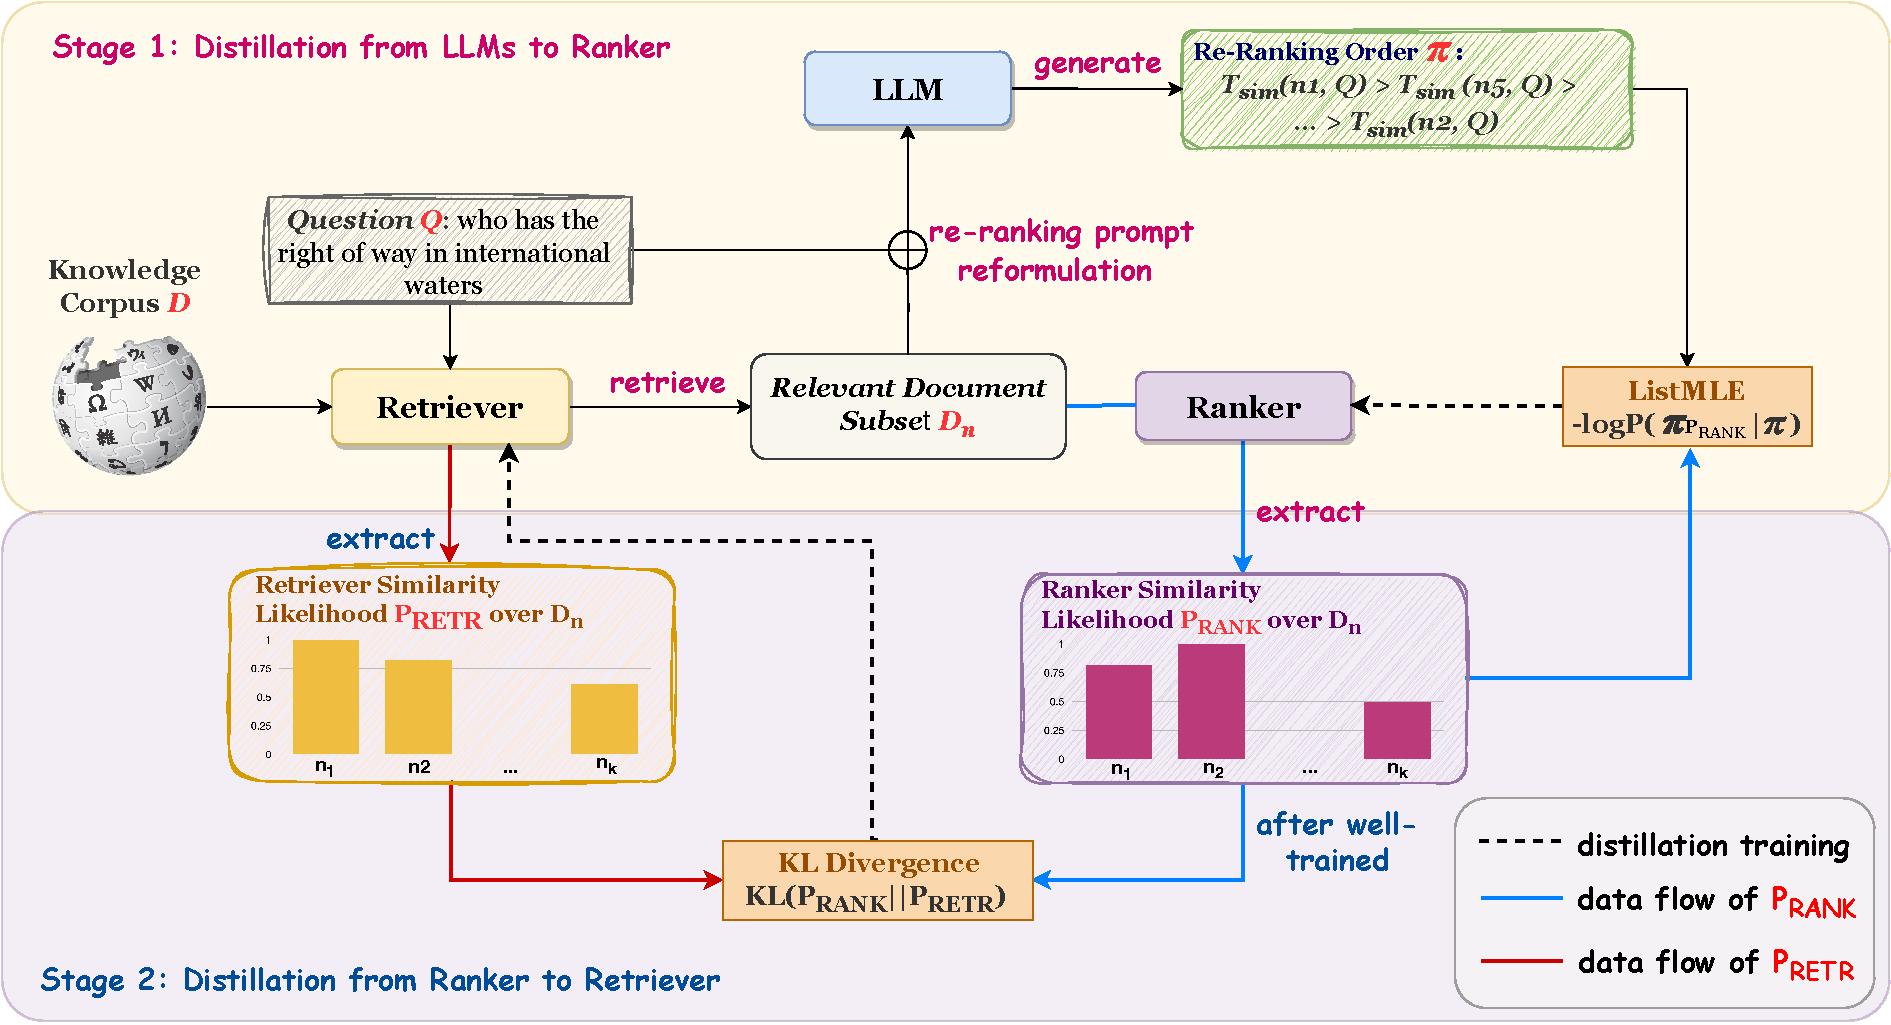
\includegraphics[width=1.0\textwidth]{latex/pic/fig2-3.pdf}
    \caption{The two-stage knowledge distillation process of our proposed Intermediate Distillation scheme. In Stage 1, we use re-ranking order $\pi$ (highlighted in the green background color) as the supervisory signal to train a ranker model. In Stage 2, this distilled ranker unsupervised trains the retriever model to enhance its performance.}
    \label{fig:02}
\end{figure*}

\subsection{Retrieval-Augmented Generation}
Information retrieval plays a crucial role in various knowledge-intensive NLP tasks, including question-answering \cite{siriwardhana2023improving, zhang2024raft}, fact-verification \cite{hang2024trumorgpt, khaliq2024ragar} and open-domain dialogue \cite{wang2024unims, shuster2021retrieval}.
A prevalent approach in information retrieval is the multi-stage retrieval process \cite{nogueira2020document}, which first uses a retriever model to search several most relevant documents from the large corpus, then employs a ranker model to further optimize the ranking order based on relevance, and returns the top few most relevant documents finally.

% For example, researchers have fine-tuned LLMs to act as retrieval or re-ranking models, which outperform the existing smaller models. 
% Moreover, it has already demonstrated that LLMs are of excellent zero-shot reranking capabilities.
% The effectiveness of the RAG framework has been validated across various NLP downstream tasks, including open domain question-answering, fact-verification and dialogue.

Recently, the retriever models are increasingly used to enhance the generation quality of LLMs for knowledge-intensive tasks due to their flexibility and effectiveness, leading to the development of the retrieval-augmented generation (RAG) framework \cite{guu2020retrieval, izacard2023atlas}.
This framework integrates information retrieval into the generation process of LLMs, which helps overcome the models' limitations, such as hallucination, by utilizing external up-to-date information. 
% This method reduces the dependency of LLMs on their internal parameters to encode world knowledge, thereby reducing the occurrence of hallucination problems in LLMs generation.
% Normally, the RAG framework consists of a retriever model and a reader model. 
% The retriever is responsible for searching the relevant information from the large corpus, while the reader combines this retrieved information with query as input and generate responses.
In the RAG framework, the retrieved information can be in the form of tokens, entities, or text chunks (i.e., documents), and the retrieval can occur once or repeatedly every $n$ tokens, for finding a balance between the performance and time-cost.
% Specifically, the retrieved information form can be tokens, entities, or text chunks (i.e., documents); the retrieval process can be performed just once, or it can be executed every $n$ tokens, which could enhance the performance but also increase the inference time cost. 
Additionally, the retrieval model in RAG is adaptable to both encoder-to-decoder \cite{guu2020retrieval, izacard2023atlas} and decoder-only language models \cite{borgeaud2022improving, ram2023context}, and is applicable during both the pre-training \cite{zhong2022training, min2022nonparametric} and inference stages \cite{menick2022teaching, min2023factscore}. 

In this paper, we use the advanced knowledge from LLMs as the supervision signal to train the retriever models through a multi-stage (i.e., rerank-then-retrieve) training scheme.
We then integrate our well-trained retriever model into the RAG framework, 
demonstrating the effectiveness of our proposed training framework in question-answering tasks.
% demonstrating that our distillation method substantially improves the performance of LLMs in question-answering downstream tasks.


\subsection{Knowledge Distillation in LLMs.} 
Knowledge distillation is widely used to transfer knowledge from complex, large teacher models to smaller student models \cite{hinton2015distilling}.
Influenced by the outstanding performance of LLMs, more and more studies focus on using LLMs as teacher models to distill knowledge into smaller task-specific models \cite{brown-etal-2023-efficient}, and the distillation methods can be categorized into two types: white-box \cite{gu2023minillm, agarwal2023gkd, udagawa-etal-2023-comparative} and black-box \cite{li2022explanations, ho2022large, hsieh2023distilling}.
Specifically, white-box training leverages both the predictions and the parameters of LLMs to exact knowledge, which can be memory-intensive and computationally demanding. 
In contrast, black-box training only relies on the predictions of LLMs, making it less resource-intensive.

Many studies have successfully integrated knowledge distillation within the RAG framework to train the retriever models.
For white-box LLM distillation training, previous researches employ LLM likelihood, such as attention scores, to assess the relevance distribution of retrieved documents \cite{izacard2023atlas, izacard2022unsupervised}.
Meanwhile, some recent studies have also explored methods for training RAG using black-box LLMs, like In-Context RALM \cite{ram2023context} and RePLUG \cite{shi2023replug}.
% This kind of methods use the LLM's output probability distribution as the supervisory signal to train the 
% They directly transfer the semantic relevance of the retrieved information to the retriever model based on the next token's prediction probability, which is assumed to be the ground truth.
The remaining problem is that these methods still rely on the generation log probabilities for the ground truth as the supervision signals in distillation training, which tend to have a degree of randomness and are limited to the availability of the output probabilities.
Furthermore, aligning LLM predictions with the goals of retriever training is not the optimal choice since there remains a gap between retrieval and generation.
% Typically, using white-box training methods require deploying LLMs locally, which is complex to implement.
% Moreover, this kind of methods consumes increasingly more computational resources as the scale of LLMs models continues to expand, making it progressively more difficult to sustain. 
% Some recent studies have proposed methods for training Retrieval-Augmented Generation (RAG) based on black-box language models.
% Currently, there are also some studies that conduct training within the Retrieval-Augmented Generation (RAG) framework based on black-box LLMs, such as in-context learning and RePLUG. 
% Generally, these output probability-based methods have more randomness, and has limited scope since the output probabilities of LLMs are not always available.
% In addition, optimizing the prediction of LLM is not always matching the goal of training a retriever model, as there has a gap between retrieval and generation process.
% the training a retrieval model to semantically align directly with LLMs also requires extensive training data.
% These methods use LLMs to generate a series of quantitative score distributions to measure how much each retrieved document could improve the LM perplexity, thereby reveal the relevance of each document to the query. 
% However, this score distribution is not stable. 

In contrast, our proposed distillation method only requires black-box LLMs to output a relevance-based ranking order of the candidate relevant documents, yielding more consistent, matching, and interpretable results than output probability-based methods.
Moreover, our method is much more data efficient, requiring about 100x and 1000x less data compared to previous approaches \cite{shi2023replug, ram2023context}, significantly saving computational resources and increasing the flexibility of the training process.



